%\title{Auto, Swap positioning of Nodes, see manual p. 191}
\documentclass[11pt]{article} % use larger type; default would be 10pt

\usepackage[utf8]{inputenc} % set input encoding (not needed with XeLaTeX)

\usepackage{tikz}
\begin{document}

%% ------------ AUTO --------------------%
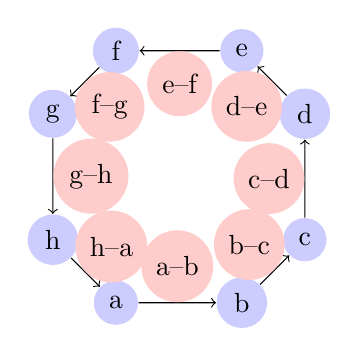
\begin{tikzpicture}
[scale=.8,
	auto=left,
	every node/.style={circle,
				      fill=blue!20}]
  \node (a) at (-1,-2) {a};
  \node (b) at ( 1,-2) {b};
  \node (c) at ( 2,-1) {c};
  \node (d) at ( 2, 1) {d};
  \node (e) at ( 1, 2) {e};
  \node (f) at (-1, 2) {f};
  \node (g) at (-2, 1) {g};
  \node (h) at (-2,-1) {h};
 
 \foreach \from/\to in {a/b,b/c,c/d,d/e,e/f,f/g,g/h,h/a}
	\draw [->] ( \from ) -- ( \to )
		node[midway,fill=red!20] {\from--\to};
\end{tikzpicture}


%% -------------- SWAP -------------------%

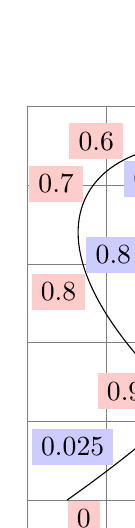
\begin{tikzpicture}[auto]
\path[ use as bounding box ] (0,0) rectangle (1,6);
  \draw[help lines,use as bounding box] (0,-.5) grid (4,5);
  \draw (0.5,0) .. controls (9,6) and (-5,6) .. (3.5,0)
  \foreach \pos in {0,0.1,0.2,0.3,0.4,0.5,0.6,0.7,0.8,0.9,1}
	 { node [ pos=\pos,swap,
			fill=red!20 ]   {\pos} }
  \foreach \pos in {0.025,0.2,0.4,0.6,0.8,0.975}
	{ node [ pos=\pos,
		        fill=blue!20 ] {\pos} };
\end{tikzpicture}

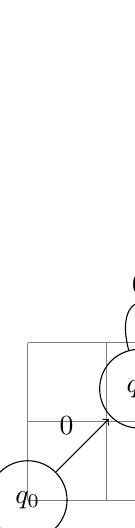
\begin{tikzpicture}[shorten >=1pt,node distance=2cm,auto,
				state/.style={circle,draw,inner sep=0pt,
									minimum size=1cm}]
\path[ use as bounding box ] (0,0) rectangle (1,6);

  \draw[help lines] (0,0) grid (3,2);
	\node[state] (q_0) {$q_0$};
	\node[state] (q_1) [above right of=q_0] {$q_1$};
	\node[state] (q_2) [below right of=q_0] {$q_2$};
	\node[state] (q_3) [below right of=q_1] {$q_3$};

  \path[->] (q_0) 
	edge node {0} (q_1)
	edge node [swap] {1} (q_2)
	(q_1) edge node {1} (q_3)
	edge [loop above] node {0} ()
	(q_2) edge node [swap] {0} (q_3)
	edge [loop below] node {1} ();
\end{tikzpicture}


\end{document}